\section{Systemtest med kendt input} \label{sec:test_kendtinput}
I dette afsnit vil det samlede system testes, således det er muligt at undersøge, om systemet behandler inputs som forventet. På baggrund af disse målinger er det muligt at konkludere, hvorvidt systemet virker. 

\subsection{Beskrivelse}
For at simulere accelerometresignaler anvendes to spændingsforsyninger til at repræsentere accelerometrene. Spændingen varieres over tid, således denne svarer til en samlet vinkel mellem $90-180^{\circ}$. Derudover testes det, om vinklen vil falde til $-200^{\circ}$ for hvert accelerometer, når spændingen svarende til $180^{\circ}$ overskrides. 

For at teste det samlede system med et kendt input benyttes en funktionsgenerator, således et $500~Hz$ sinussignal med en peak-peak-amplitude på $4~mV$ kan genereres. Sinussignalets frekvens og amplitude er omkring, hvad der kan forventes af et EMG-signal. Outputtet fra sinussignalet er filtreret gennem det implementerede digitale lavpasfilter. 

Testen foretages over 10 sekunders måling og samples via mikrokontrolleren. Ud fra disse målinger, er det muligt at teste systemets blokke, når de er sammensat. Dette gøres ved at sammenligne input og output af det samplede sinussignal samt spændingerne for acclerometrene omregnet til en samlet vinkel.


\subsection{Resultater af test}
Fra testen plottes og visualiseres systemets input af det samplede sinussignal, output fra det opsamlede digitalt filtrerede signal samt spændingen fra de to accelerometre, der er omregnet til en samlet vinkel ved lineær interpolation. Derudover er det opsamlede digitale output, som er behandlet i EMG-algoritmen, plottet. Resultaterne fremgår af \autoref{fig:test_kendtinput}. 

\begin{figure}[H]
\centering
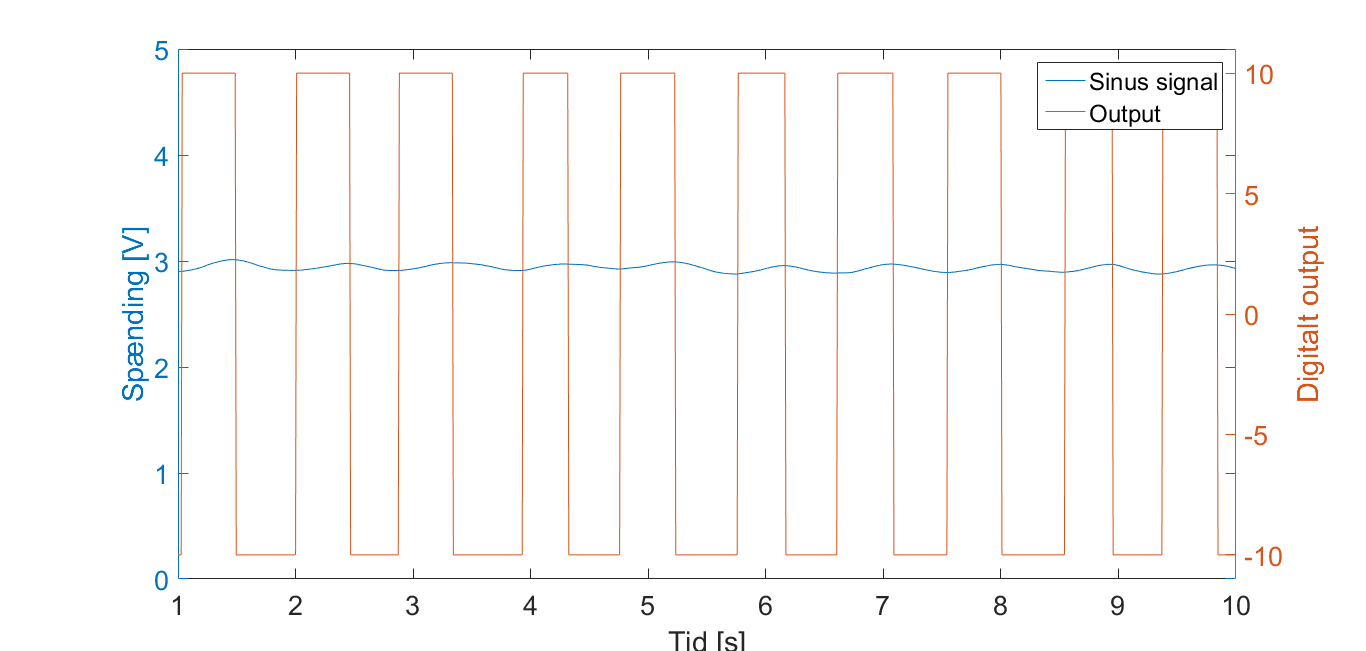
\includegraphics[width=1\textwidth]{figures/kontrol_test_sinus}
\caption{På den øverste graf illustreres den samlede vinkel over tid. Det fremgår af grafen, at vinklen er stigende fra $90^{\circ}$ til $175^{\circ}$, hvorefter vinklen falder til $-115^{\circ}$. Dette skyldes en overskridelse af spændingen for accelerometeret svarende til $180^{\circ}$.
På den midterste graf illustrerer den blå graf det opsamlede inputsignal, svarende til en sinus på $500~Hz$ med en $V_{pp}$ på $4~mV$. Den røde graf illustrerer det samplede sinussignal med et implementeret digitalt lavpasfilter, disse værdier er målt i spænding. 
På den nederste graf illustreres signalets digitale output. Signalet går fra $+10$ ved stigende muskelaktivitet til $-10$ ved en faldende muskelaktivitet. Grafen går i $0$, når en vinkel udenfor $90-180^{\circ}$ opnås.}
\label{fig:test_kendtinput}
\end{figure}

\noindent
På baggrund af målingerne for den øverste graf på \autoref{fig:test_kendtinput} fremgår det, at en indsendt stigende spænding svarende til $90-175^{\circ}$, får det den samlede vinkel til at stige. Ved en vinkel på $175^{\circ}$ overskrider det ene accelerometer dens maksimale spænding, hvorfor vinklen falder til $-115^{\circ}$ over $1~ms$. 

Dette burde ifølge den implementerede kode gå ned til en vinkel på $-200^{\circ}$ ved overskridelse af vinklerne, hvori EMG-algoritmen fungerer. 
At vinklen ikke når en samlet værdi på $-400^{\circ}$ er en indikatior for, at det ene accelerometers spænding har været inden for algoritmens grænser, mens det andet accelerometer har overskredet grænserne. Hertil kan det ses, at det ene accelerometer har haft en outputspænding svarende til $85^{\circ}$, mens det andet accelerometer har haft en spænding, der har overskredet grænsen og derfor har en vinkel på $-200^{\circ}$.

Det fremgår af den midterste og nederste graf på \autoref{fig:test_kendtinput}, at der ses en sammenhæng mellem det opsamlede digital filtrerede sinussignal og det opsamlede outputsignal. Ved et stigende sinussignal vil outputsignalet indikere $+10$, hvilket svarer til en positiv hældning af sinussignalet. Ved en negativ hældning af sinussignalet vil outputsignalet indikere et fald og dermed give et output på $-10$.

På den nederste graf på \autoref{fig:test_kendtinput} fremgår det, at efter outputsignalet har befundet sig i $-10$ ved $9~s$, stiger outputsignalet efterfølgende til $0$. Dette er grundet, at de samlede grader har overskredet én eller flere grænser, og derved fungerer EMG-algoritmen ikke, hvilket illustreres ved, at outputsignalet er $0$.

Der er yderligere foretaget en test af det samlede forsinkelse på systemet uden trådløs kommunikation. Denne test blev udført på samme måde som i \autoref{sec:lavpas_test}. Resultaterne for forsinkelse blev målt til $832~\mu s$ for det samlede system testet uden trådløs kommunikation. 